\documentclass[11pt, parskip=half]{scrartcl}
\usepackage{unicode-math}
\setmathfont{TexGyreSchola-Math}
\usepackage{naughtyornice}
\usepackage{caption}
\usepackage{subcaption}
\usepackage{ragged2e}
\usepackage{contour}

\usepackage[margin=0.43in, paperheight=5.25in, paperwidth=3.75in]{geometry}

% Minimize unwanted hyphenation
\tolerance=1
\emergencystretch=\maxdimen
\hyphenpenalty=1
\hbadness=10000

\usepackage{eso-pic}
\usepackage{booktabs}

\setkomafont{section}{\setmainfont{Berkshire Swash}\LARGE\color{XmasGreen}}
\setkomafont{subsection}{\setmainfont{Berkshire Swash}\Large\color{XmasGreen}}
\setkomafont{subsubsection}{\setmainfont{Berkshire Swash}\large\color{XmasGreen}}

% Adjust spacing before and after section headings
\RedeclareSectionCommand[
  runin=false,
  beforeskip=0.5\baselineskip,
  afterskip=-0.0\baselineskip
]{section}

% Adjust spacing before and after subsection headings
\RedeclareSectionCommand[
  runin=false,
  beforeskip=0.5\baselineskip,
  afterskip=-0.0\baselineskip
]{subsection}

% Adjust spacing before and after subsubsection headings
\RedeclareSectionCommand[
  runin=false,
  beforeskip=0.5\baselineskip,
  afterskip=-0.0\baselineskip
]{subsubsection}


\usepackage{enumitem}

\usepackage[hang,flushmargin]{footmisc}
\newcommand\blfootnote[1]{%
  \begingroup
  \renewcommand\thefootnote{}\footnote{#1}%
  \addtocounter{footnote}{-1}%
  \endgroup
}

\renewcommand{\thefootnote}{\fnsymbol{footnote}}
\renewcommand{\footnoterule}{%
  \kern -3pt
  \hrule width \textwidth height 0.5pt
  \kern 2pt
}

\usepackage[hidelinks]{hyperref}
\usepackage[type={CC}, version={4.0}, modifier={by-sa}]{doclicense} % Add text and icons for creative commons license
%\usepackage{array}

\raggedright
\pagestyle{empty}
\begin{document}

\begin{titlepage}
\pagecolor{white}
\AddToShipoutPictureBG{
\begin{tikzpicture}[remember picture, overlay]
%	\node () at (current page.center) {\includegraphics[width=\pagewidth, height=\pageheight]{Images/aloft_cover_background.png}};
%	\node () at (current page.center) {\includegraphics[width=\pagewidth, height=\pageheight]{Images/dessert_dice_front_cover_compressed.jpg}};
\end{tikzpicture}
}

\enlargethispage{1.25\baselineskip}
\setmainfont[Scale=2.2]{Berkshire Swash}
\Huge
\begin{center}
\textcolor{XmasRed}{Naught\hspace{0.125ex}y}

\textcolor{black!70}{or}\ \,\textcolor{XmasGreen}{N\hspace{0.2ex}ice}

\vfill

\begin{tikzpicture}
\node[inner sep=0pt] at (0,0) {
\includegraphics[scale=0.06]{Images/gingerbread_man_yellow.png}};
\node[inner sep=0pt] at (0:0.95in) {
\includegraphics[scale=0.06]{Images/tree_cookie2_yellow.png}};
\node[inner sep=0pt] at (180:0.95in) {
\includegraphics[scale=0.06]{Images/gingerbread_tree_yellow.png}};
\node[inner sep=0pt] at (60:0.95in) {
\includegraphics[scale=0.06]{Images/snowman_yellow.png}};
\node[inner sep=0pt] at (240:0.95in) {
\includegraphics[scale=0.06]{Images/santa_yellow.png}};
\node[inner sep=0pt] at (120:0.95in) {
\includegraphics[scale=0.06]{Images/ornament_yellow.png}};
\node[inner sep=0pt] at (300:0.95in) {
\includegraphics[scale=0.06]{Images/mug_man_yellow.png}};
\end{tikzpicture}

\vfill

\setmainfont[Scale=2.75]{Berkshire Swash}
\tiny
\textcolor{XmasGreen}{Designed by\ \ Michael\ Purcell}
\end{center}
\end{titlepage}
\pagecolor{white}

\setmainfont{Tex Gyre Schola}
\ClearShipoutPicture
%\enlargethispage{1.75\baselineskip}

\section*{Overview}
Naughty or Nice is a find-the-match game for two players. It can be played in about five minutes and is intended for players who are at least ten years old.

\section*{Components}
\begin{itemize}[leftmargin=*, nosep]
  \item 18 two-sided cards 
\end{itemize}

\vfill
     
      \begin{figure}[ht]
      \centering
      \subcaptionbox*{8 target cards}[0.4\textwidth]{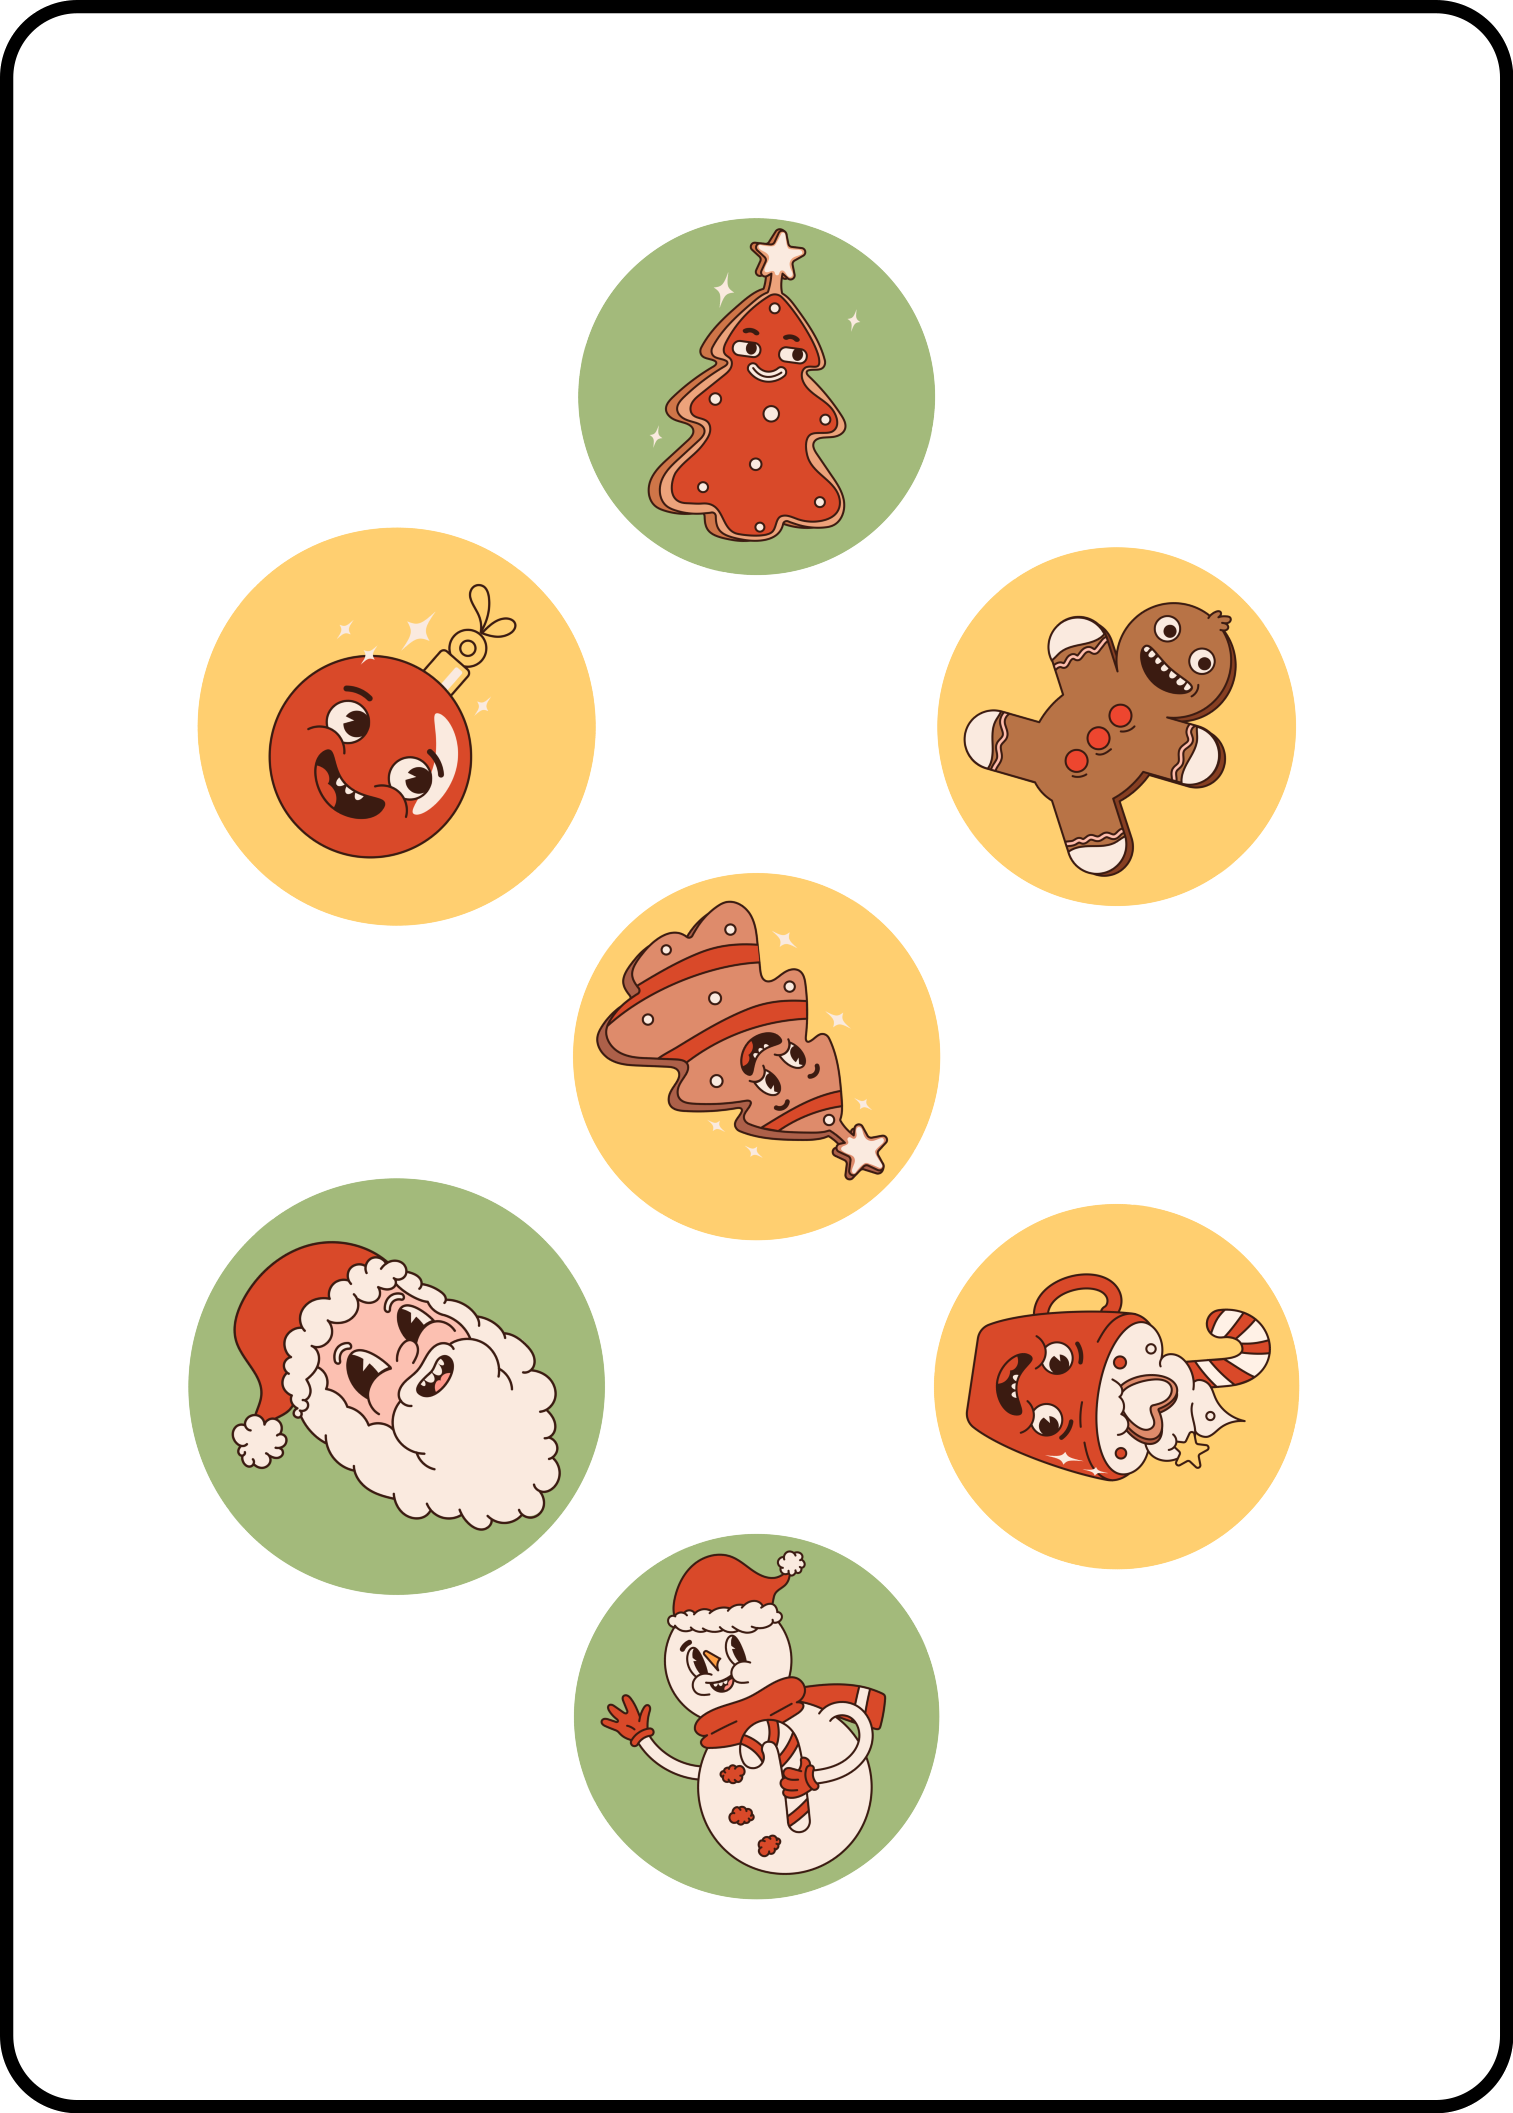
\includegraphics[scale=0.25]{Images/target_card_1_display.png}}\qquad
      \subcaptionbox*{7 character cards}[0.4\textwidth]{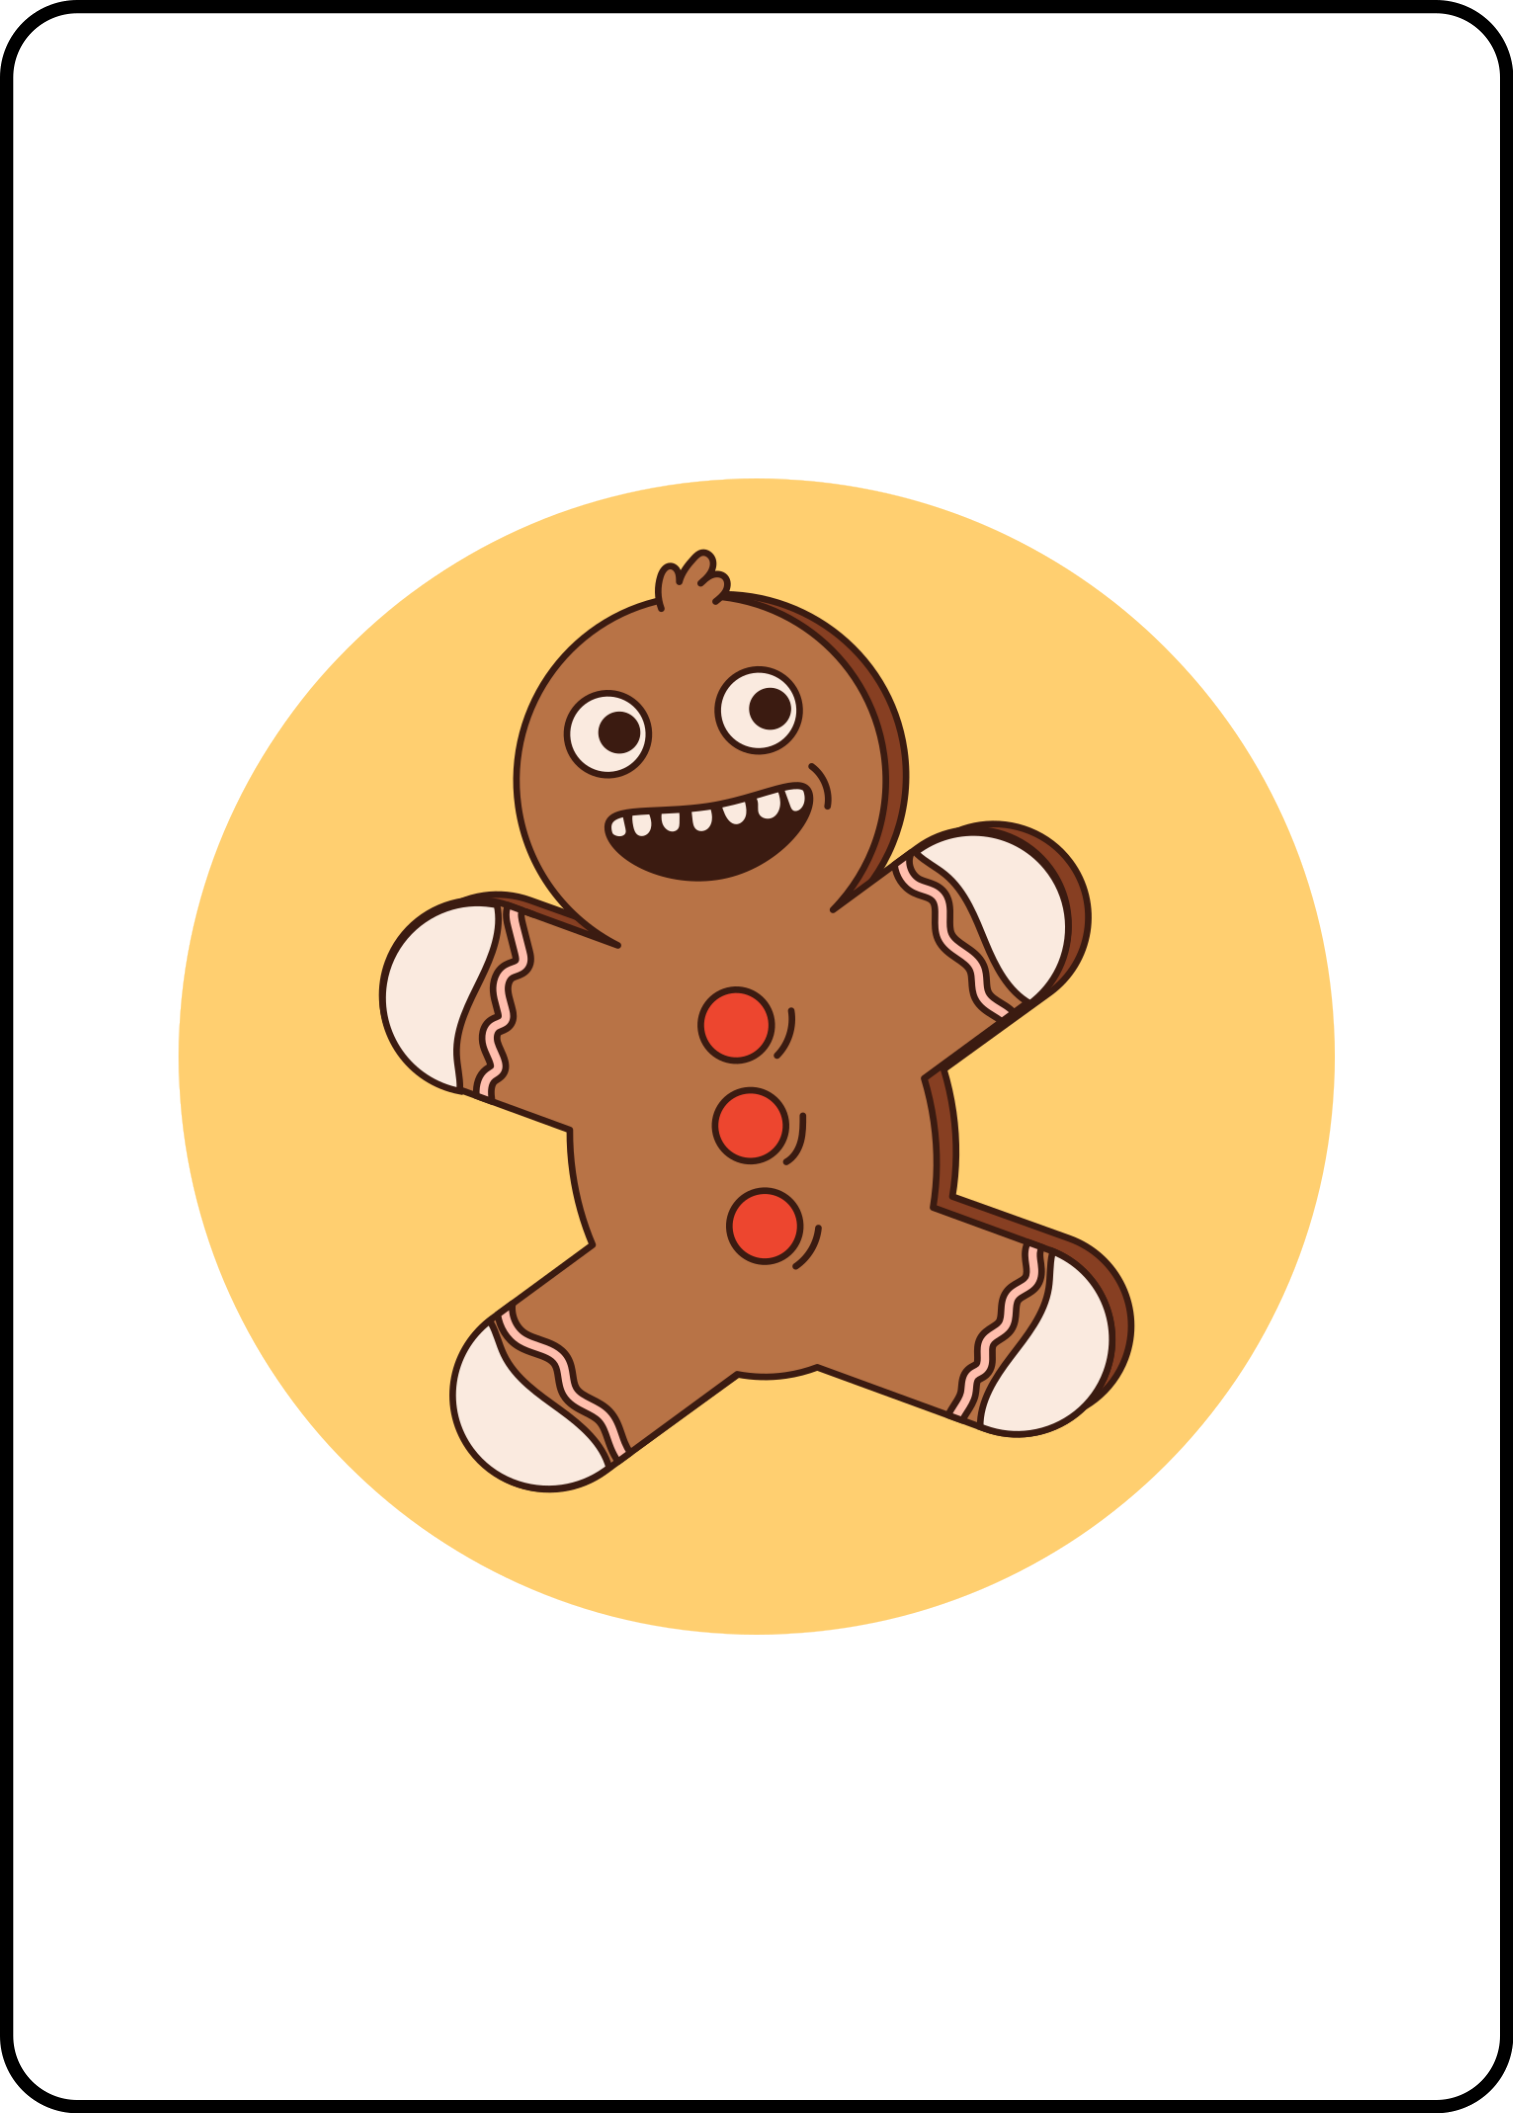
\includegraphics[scale=0.25]{Images/gingerbread_man_card_display.png}}
      \end{figure}
      
      \vfill
	  \begin{figure}[ht]
	  \centering      
      \subcaptionbox*{3 scoring cards}[0.8\textwidth]{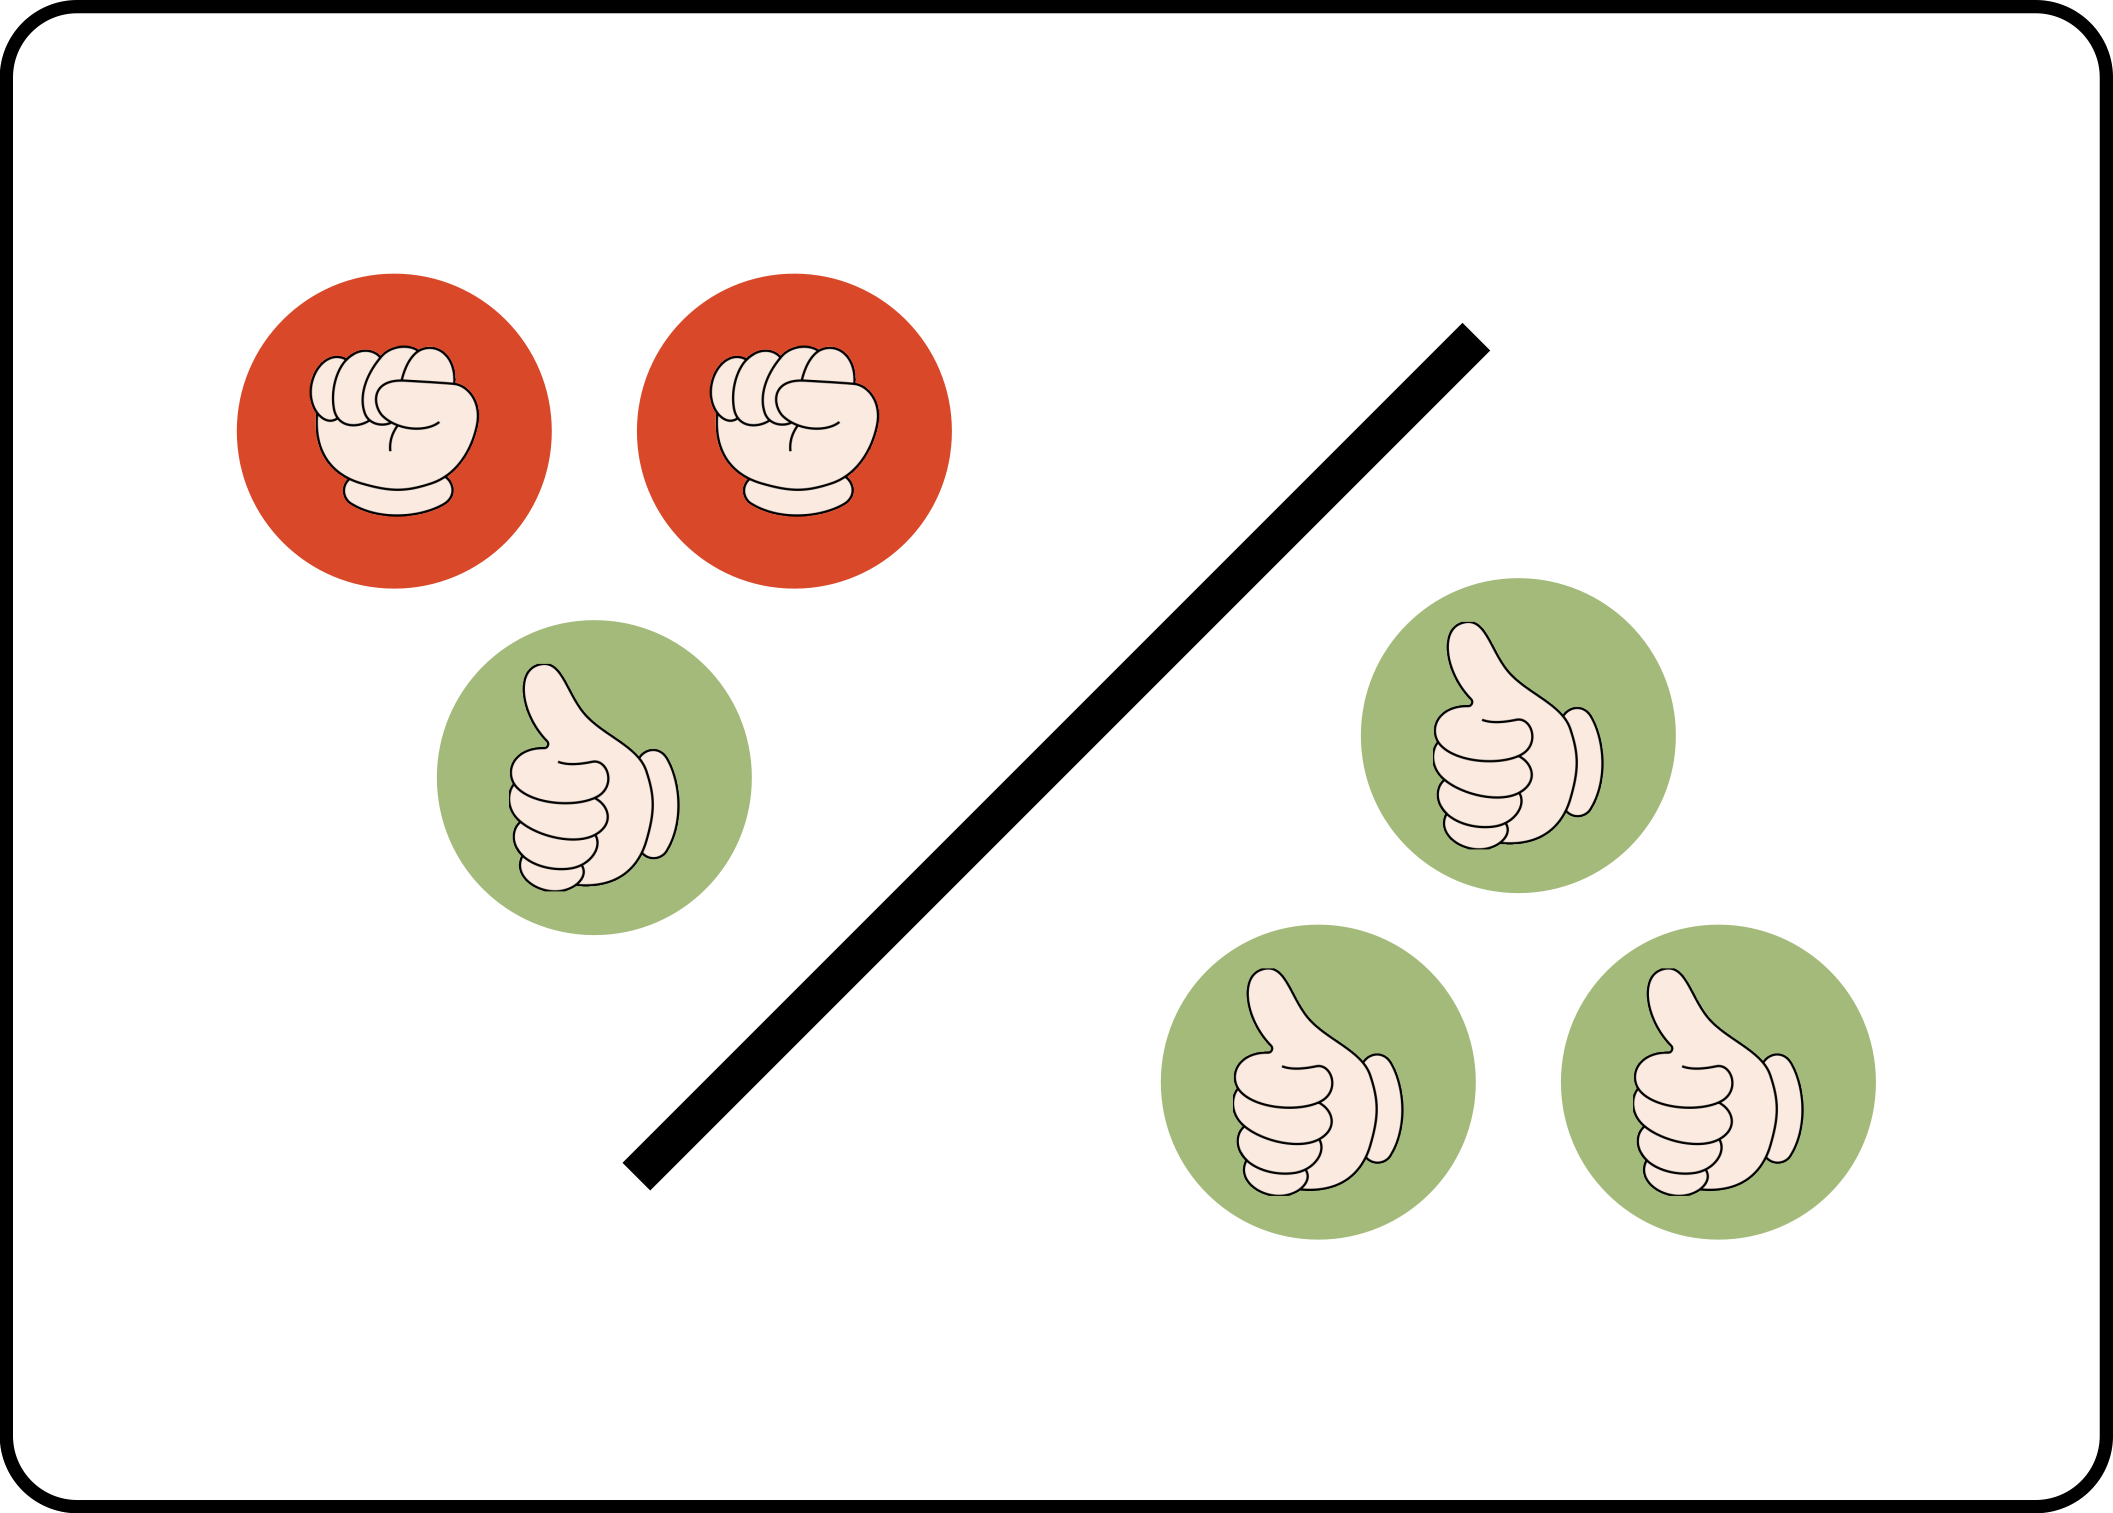
\includegraphics[scale=0.25]{Images/score_card_display.png}}  
      \end{figure}
            
\newpage

\section*{Set Up}
\begin{enumerate}[leftmargin=*]
  \item Prepare three decks of cards. Each deck will consist of all of the cards of a given type.
  \begin{itemize}[leftmargin=*]
  	\item Shuffle the target cards together to create the \emph{target deck}.
  	\item Shuffle the character cards together to create the \emph{character deck}.
  	\item Shuffle the scoring cards together to create the \emph{scoring deck}.
  \end{itemize}
  \item Place the scoring deck to one side of the play area where both players can see it easily.
  \item Place the character deck in the middle of the play area.
  \item Deal three cards from the target deck to the play area just below the character deck. 
 \end{enumerate}
 
\newpage
%\enlargethispage{1.75\baselineskip}
\section*{Gameplay}
During the game, you will compete to determine whether each of the characters are ``Naughty'' or ``Nice''.

Review the target and scoring cards in combination with each character to determine your answer and yell it out before your opponent.

If you're right, you will collect the character card and score one point. If you're wrong, your opponent will collect the card and score a point instead.

Continue like this until the character deck is exhausted. Whoever collected the most character cards wins the round and collects the scoring card.

Reshuffle the character and target decks and deal out the cards for another round. The first player to collect two scoring cards wins the game. 

\subsection*{Questions and Answers}
As you play, you will need to answer questions about the portraits displayed on the character cards.

For each character, you will need to determine if the background color behind their portrait satisfies the criterion defined by the target cards and the scoring card for that round.

If so, then the correct answer for that character is ``Nice''. Otherwise, the correct answer is ``Naughty''.

%\subsection*{Scoring Criteria}
%The target cards and scoring cards work together to define the scoring criteria for each round.

\begin{center}
\begin{tikzpicture}
\node[inner sep=0pt] at (0,0) {
\includegraphics{Images/gold_star.png}};
\node[inner sep=0pt] at (1.1in,-0.5in) {
\includegraphics[scale=0.6]{Images/gold_star.png}};
\node[inner sep=0pt] at (1.9in,0.25in) {
\includegraphics[scale=0.8]{Images/gold_star.png}};
\node[inner sep=0pt] at (0.8in,0.5in) {
\includegraphics[scale=0.4]{Images/gold_star.png}};

\end{tikzpicture}
\end{center}
\newpage
%\enlargethispage{1.75\baselineskip}


\subsubsection*{Target Cards}
The portrait of each character appears on each target card with one of two possible background colors, yellow or green.

There are three target cards in each round. So, each character card will match 0, 1, 2, or 3 of the target cards.

\subsubsection*{Scoring Cards}
%The icons displayed on the scoring card for each round determines which of the possible counts correspond to ``Nice'' and which correspond to ``Naughty''.

One side of each scoring card indicates that the even counts, that is 0 or 2, correspond to ``Nice'' while the other counts correspond to ``Naughty''.

The other side of each scoring card indicates that odd counts, that is 1 or 3, correspond to ``Nice'' while the other counts correspond to ``Naughty''.


\newpage
%\enlargethispage{1.75\baselineskip}

\subsubsection*{Example}
Consider the following situation:

      \begin{figure}[ht]
      \centering
      \subcaptionbox*{\scriptsize Scoring card}[0.3\textwidth]{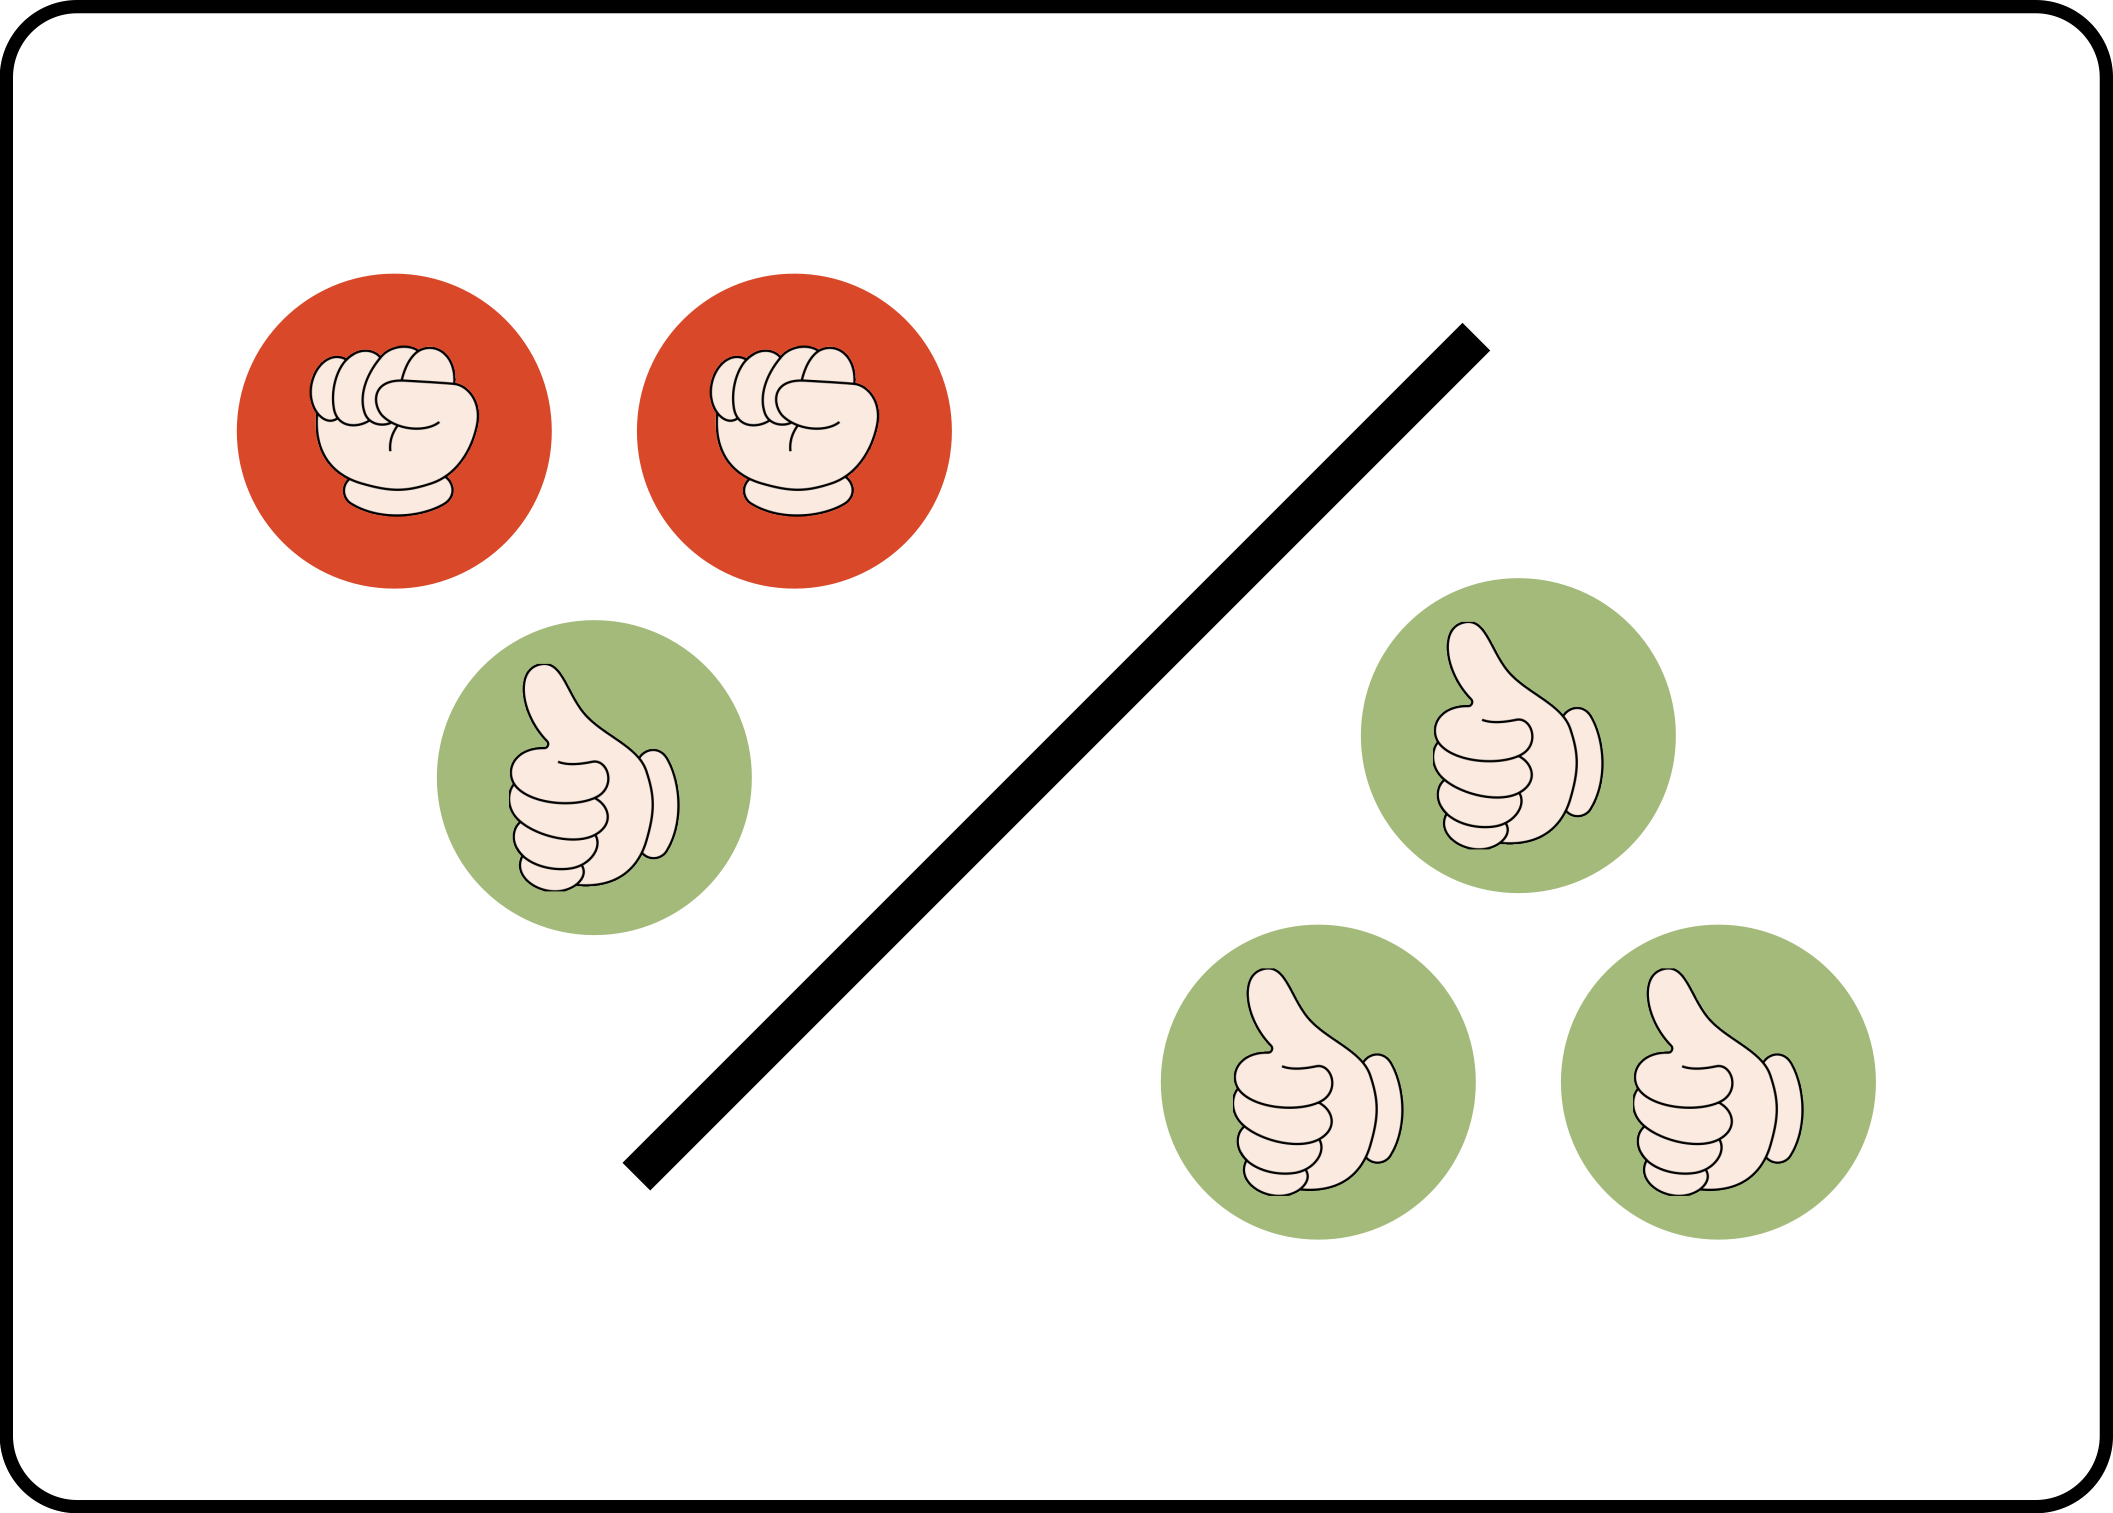
\includegraphics[scale=0.15]{Images/score_card_display.png}}
      \subcaptionbox*{\scriptsize Character card}[0.3\textwidth]{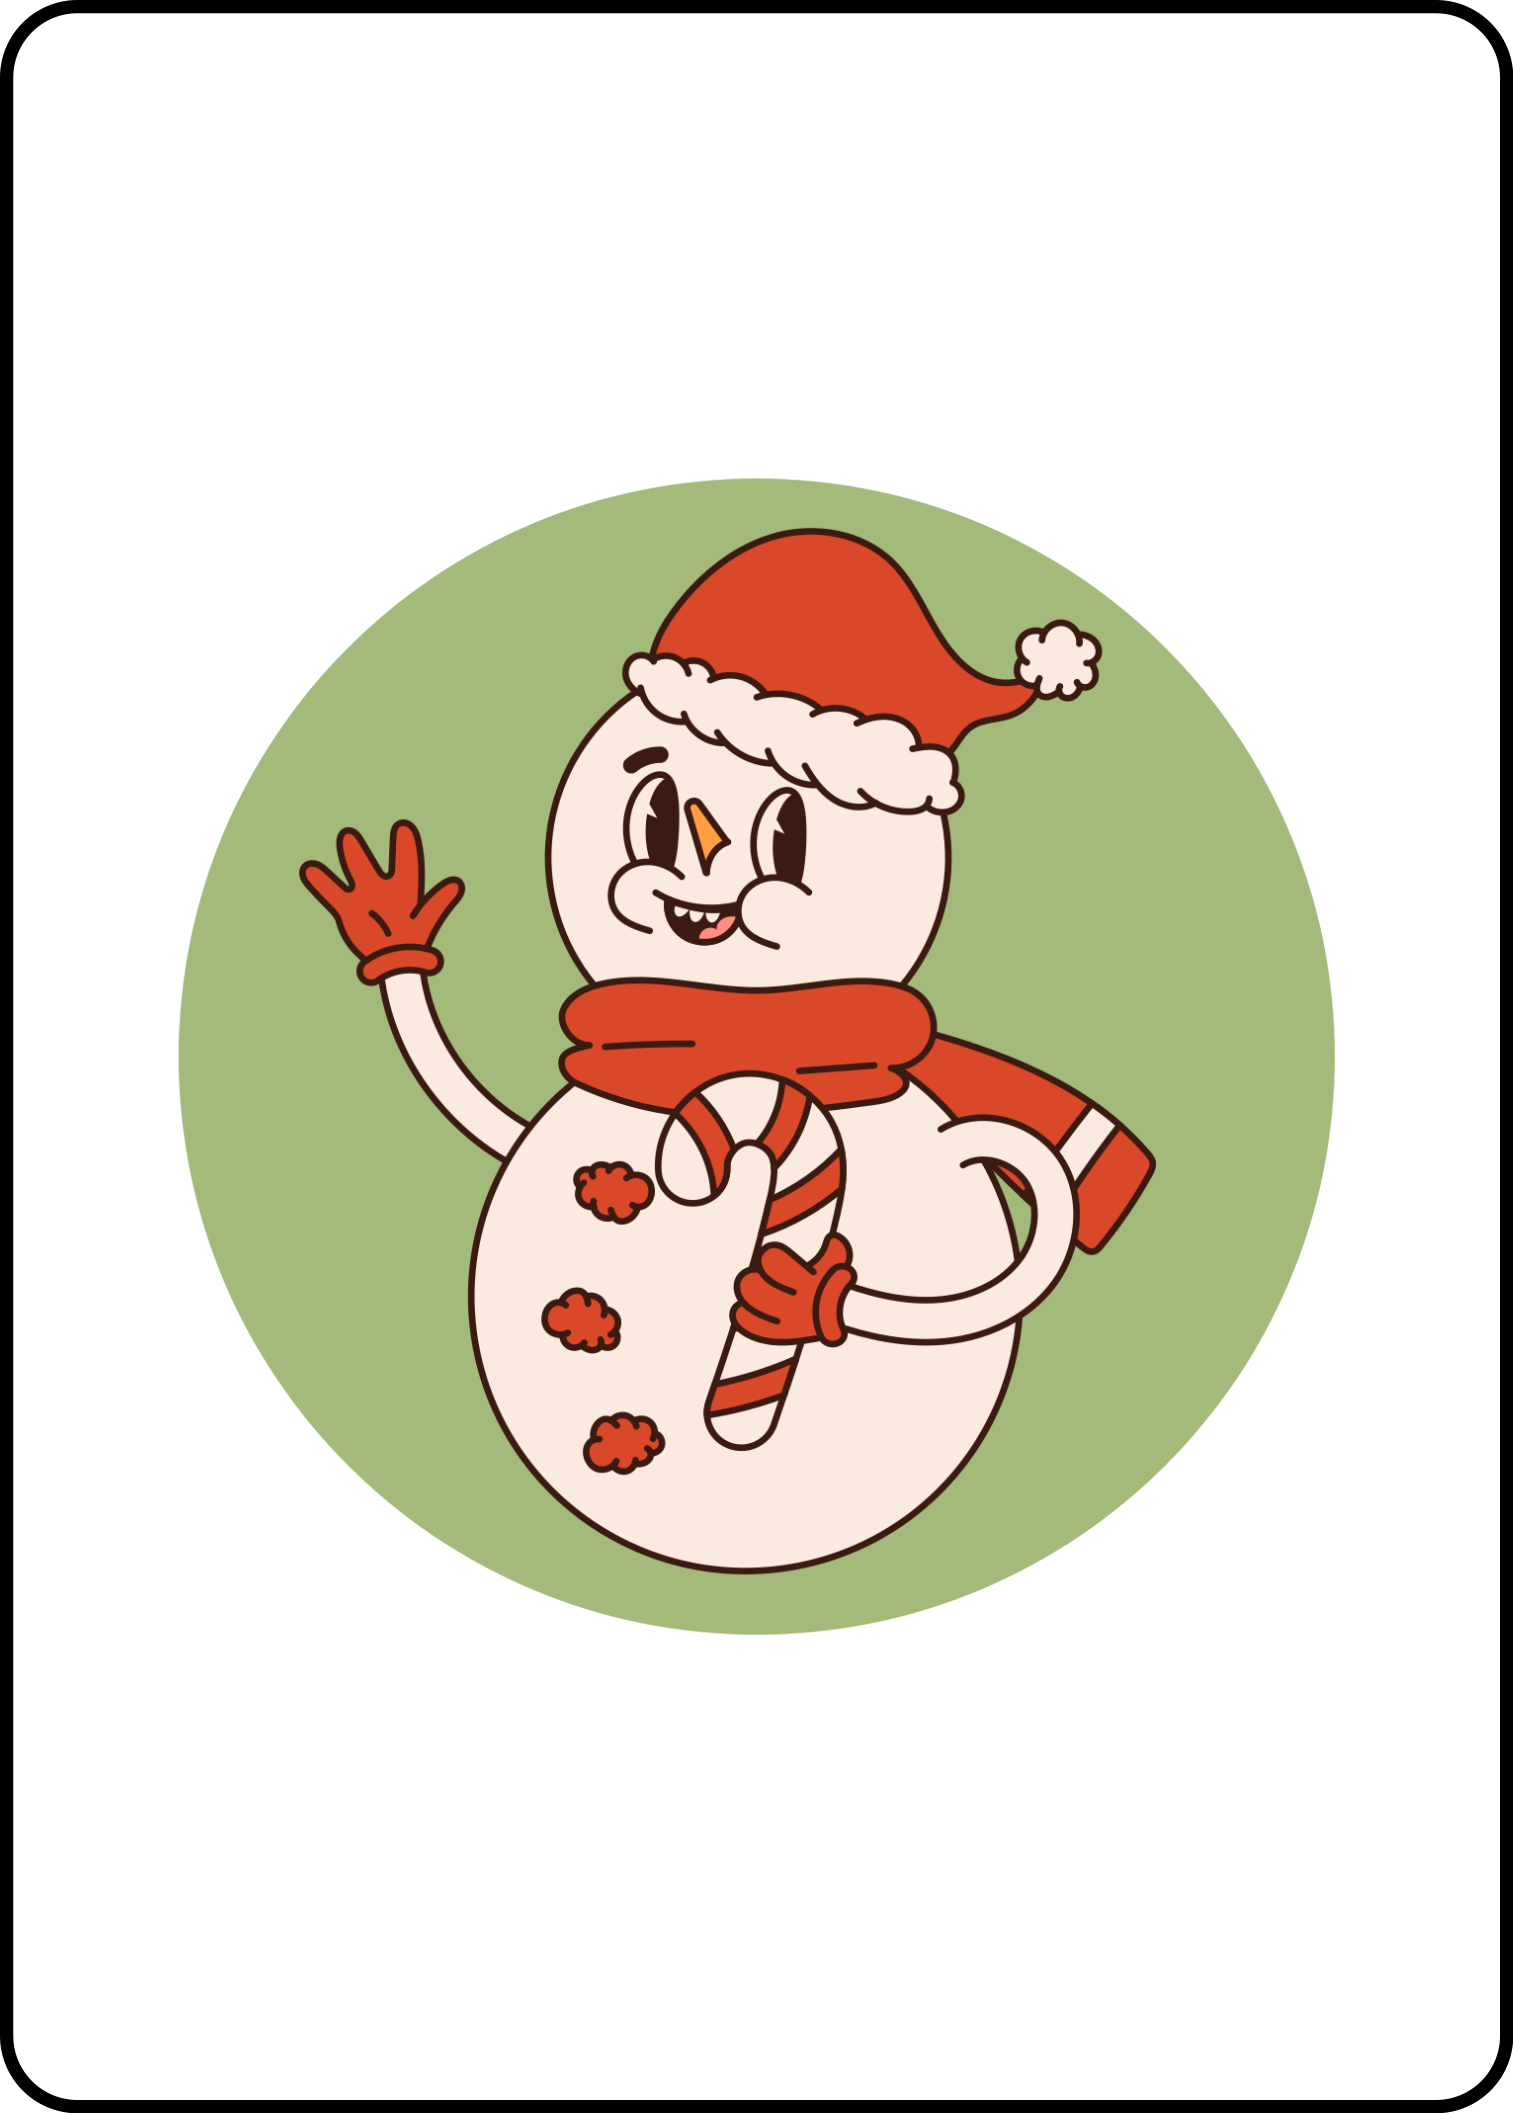
\includegraphics[scale=0.15]{Images/snowman_card_display.png}}

		\vspace{\baselineskip}      
      
      \subcaptionbox*{\scriptsize Target cards}[0.8\textwidth]{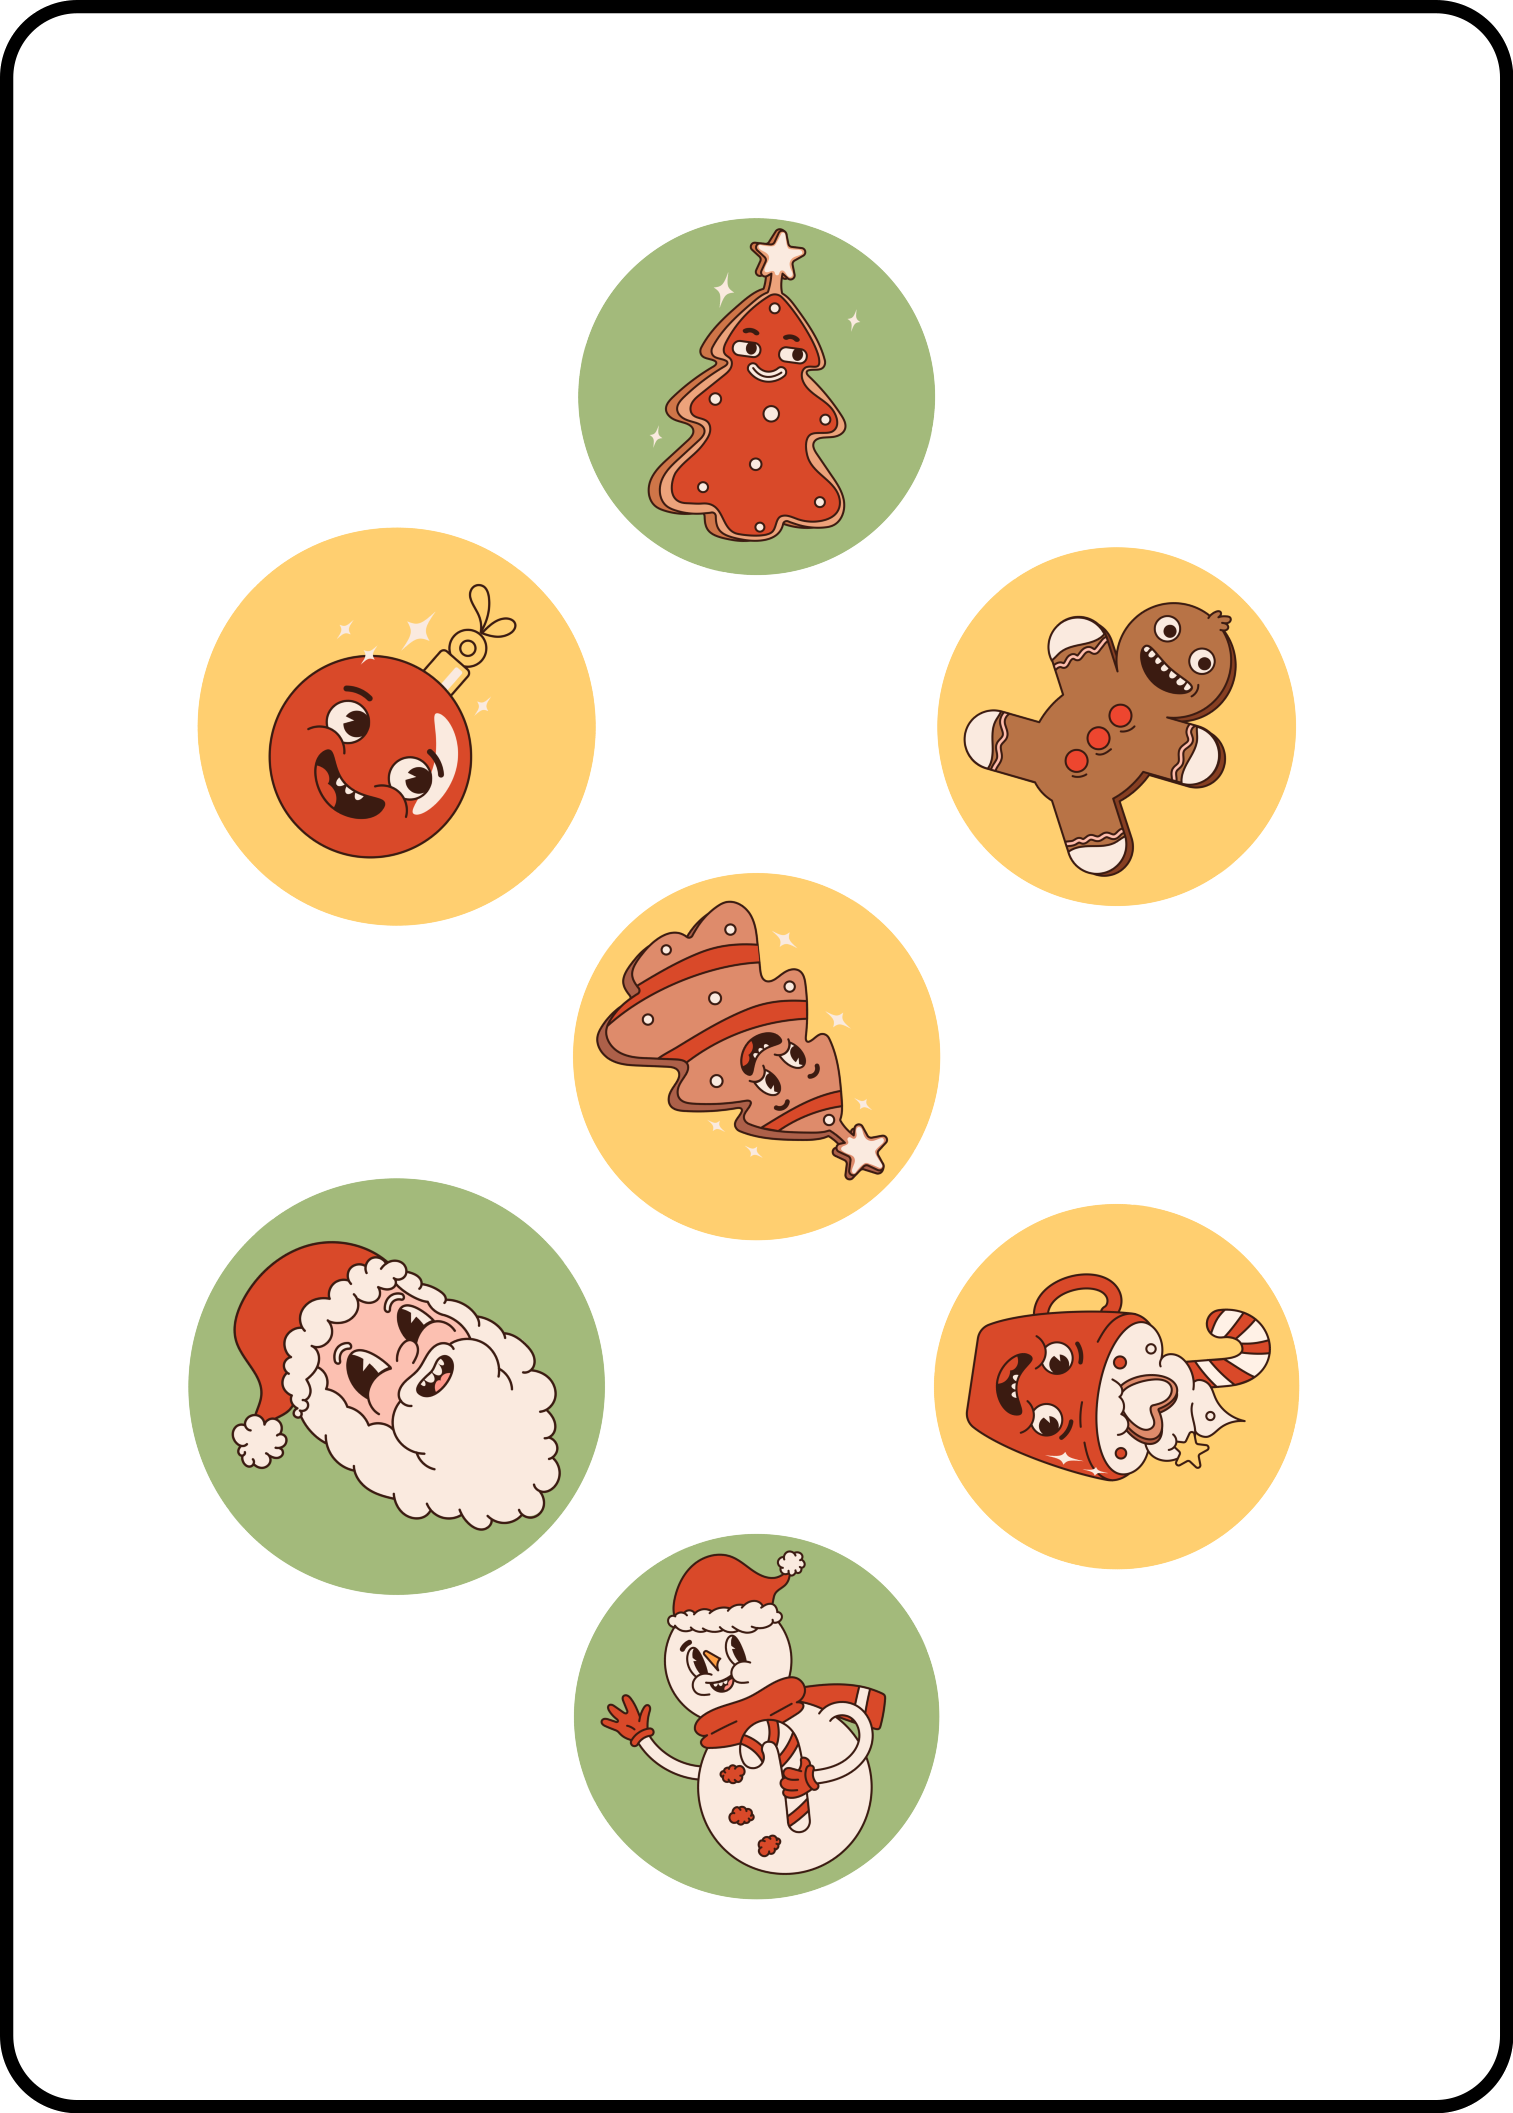
\includegraphics[scale=0.15]{Images/target_card_1_display.png} \quad 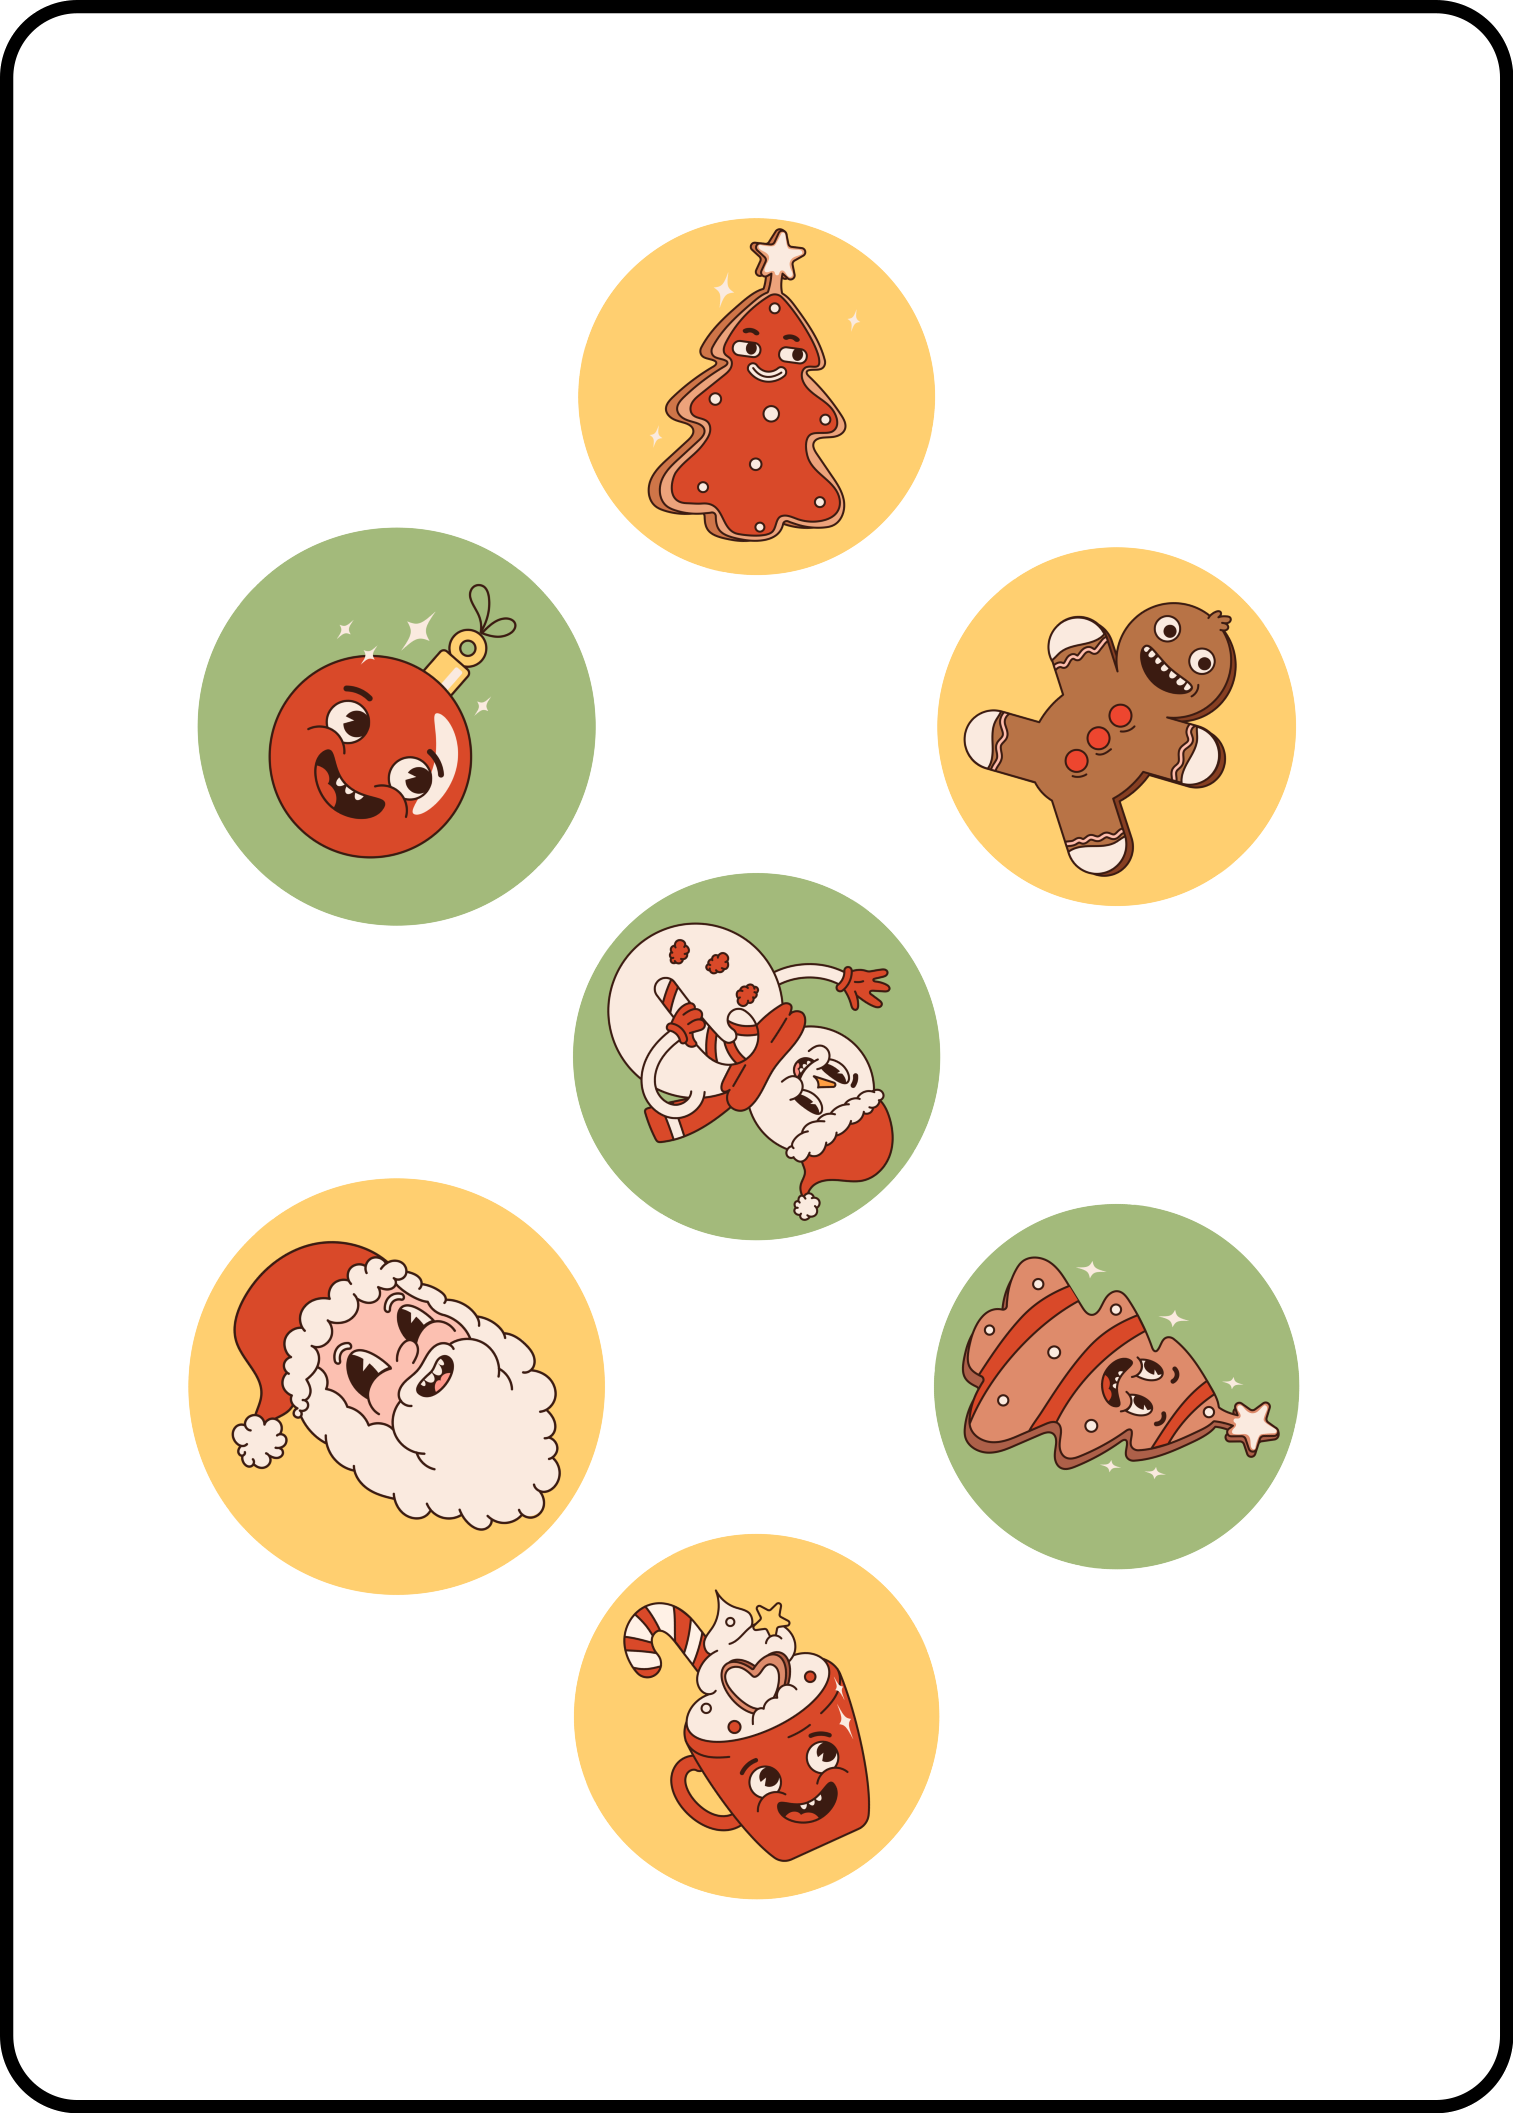
\includegraphics[scale=0.15]{Images/target_card_2_display.png} \quad 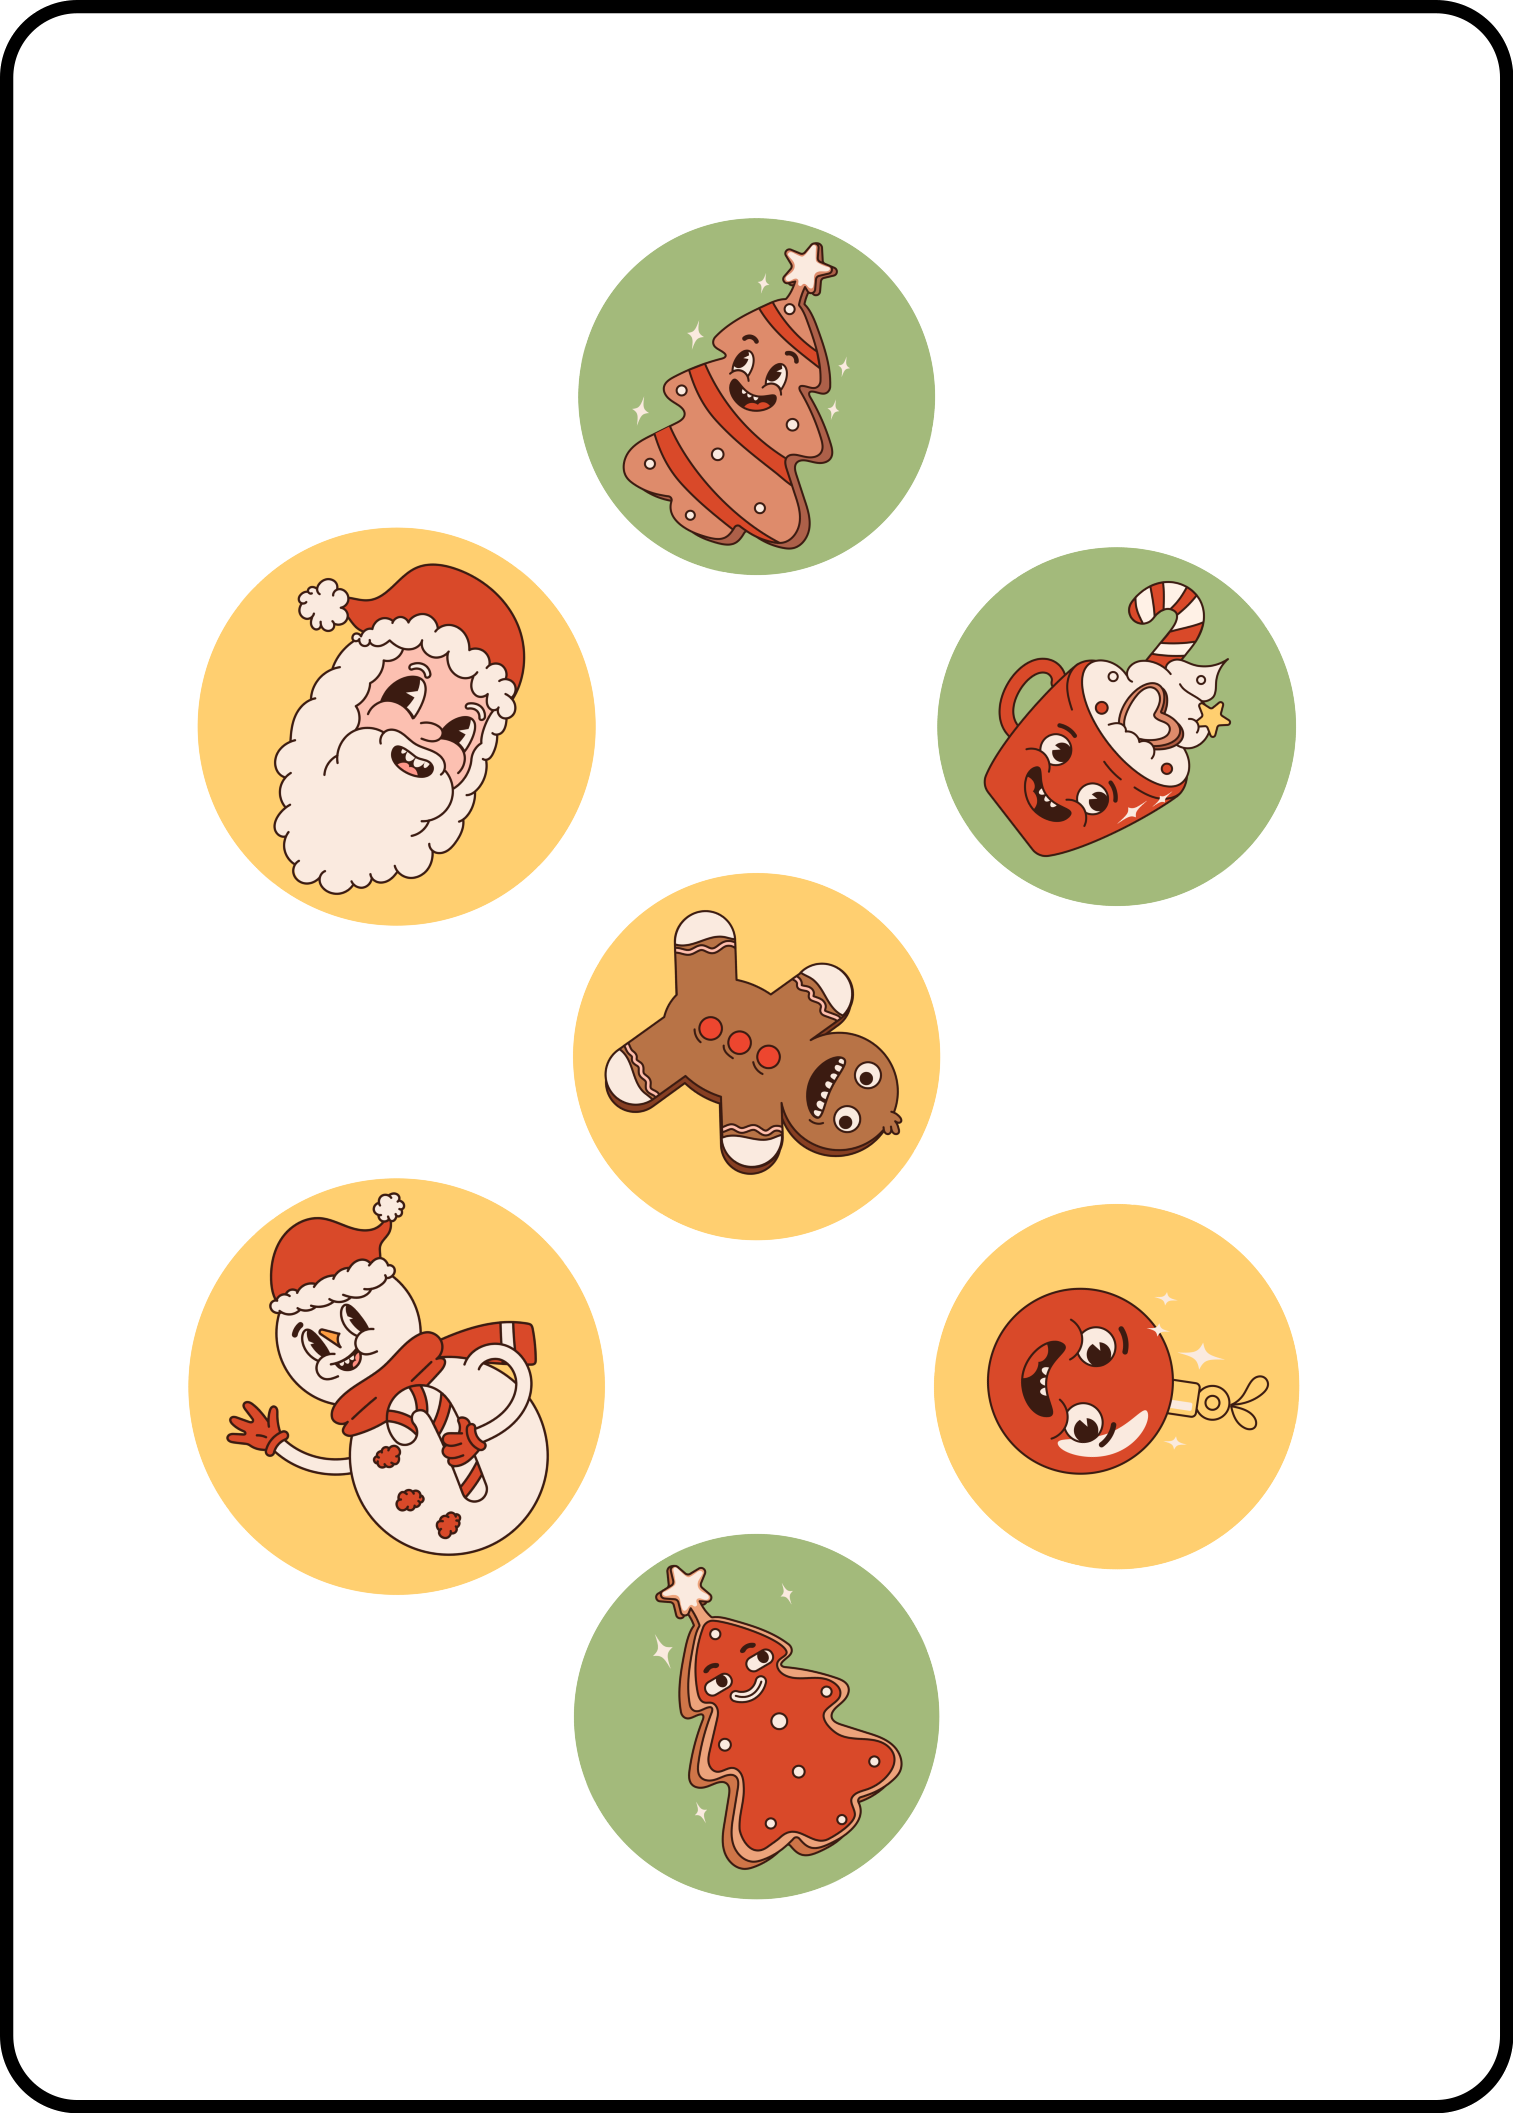
\includegraphics[scale=0.15]{Images/target_card_3_display.png}}

      \end{figure}
      
      \vspace{-0.5\baselineskip}
      
Two target cards have a snowman with a green background. So, the count is 2.

The scoring card indicates that odd counts are ``Nice''. So, the snowman with a green background is ``Naughty''.

\vspace{-1ex}

\hrulefill

\small
\textbf{Design}: Michael Purcell\\
\textbf{Contact}: \href{mailto:ttkttkt.game@gmail.com}{ttkttkt@gmail.com}\\
\textbf{License}: This work is licensed under a\\\phantom{\textbf{License}: }``CC BY-SA 4.0'' license.%\raggedright\doclicenseText

\end{document}